\chapter{Methodology}

%% \textbf{This section should include a recipe of what you did (explain what you have done so if someone wants to reproduce the experiment, they can).  A flow chart is typically helpful.  Also, make sure to define all software that you used including version numbers and OS.  Should also include a description of statistical methods used (if any).  \footnote{For more information see: \url{http://rc.rcjournal.com/content/49/10/1229.short}}}
We focus our hypernym discovery efforts on projection learning techniques.  In contrast to efforts undertaken to compare vector-combination supervision and unsupervised methods across the same corpus, datasets and evaluations metrics \citep{shwartz2017siege, roller2014inclusive, levy2015supervised}, the literature pertaining to \textit{projection learning} is fractured.  The experiments described in this section are motivated by two objectives.  

Firstly, we wanted to normalise the experimental conditions of the published methods such that they can be compared using the same methodology and metrics.  Some of the work claims that novelties introduced by the respective authors leads to improvement but the experiments were executed on a single fold of the dataset and no test results for statistical significance were provided \citep{Fu2014, ustalov2017negative, yamane2016distributional}.  In \citeauthor{yamane2016distributional}'s case, the joint-learning mechanism was deemed to be superior to \citeauthor{Fu2014}'s hard-clustering "pipeline" method but experiments on the English language were only executed on a single dataset, whereas we are working on a larger, combined dataset.  Similarly, different metrics were used in different studies which makes it impossible to compare performance differences.  Lexical memorisation was acknowledged in \cite{espinosa2016supervised} but no study attempted to train and evaluate models on lexically-split datasets.  Other than \cite{espinosa2016supervised} who used sense-disambiguated vectors \citep{iacobacci2015sensembed}, all other studies employed word2vec embeddings.  We wanted to examine the performance of the models when a transformation matrix was learned on different pre-trained embeddings of the same dimensions.  

For each model, we will be testing the effect of several hyperparameters on the final score.  Since we have several factors, with several levels associated to each factor, we will employ the $N-$way \ac{ANOVA} framework to test for significance among the interaction of several factors at 95\% confidence.  If a significant difference of means is found among factor interactions, we will proceed to run one or more post-hoc tests using Tukey's \ac{HSD} test which compares multiple pairs of means for significant differences.

The second objective is to test our projection learning understanding on the SemEval-2018 Task 9 challenge \citep{camacho2018semeval}.  This time, we focus on CRIM's soft-clustering algorithm \citep{bernier2018crim} inspired by \citeauthor{yamane2016distributional}.  We attempt to introduce some observations made from the introductory round of experiments into the models we evaluate on the shared task data.  We also exploit the shared task's particularities when designing the experiments.  For instance, query terms are subdivided into named entities and common concepts which allows us train two separate models on words belonging to each category, as well as a single model trained on both word types.  We train the models using three different embedding spaces, with vectors of larger dimension than attempted by CRIM \citep{bernier2018crim}.  Finally, we experiment with embeddings tuning motivated by \cite{howard2018universal} which yields results comparable (albeit inferior) to CRIM.  

%% Use this in evaluation:
%%The latter also tuned their embeddings to amplify their results but employed a different mechanism to ours. The paper's space constraints inhibited  \citeauthor{bernier2018crim} from describing how they tuned the embeddings.  Efforts to reproduce their method in our code yielded negative results.

\section{Hard-Clustering and Regularisation} \label{ustalov_experiment}
For this set of experiments, we leverage \citeauthor{ustalov2017negative}'s open-source code, publicly available on GitHub\footnote{\url{https://github.com/nlpub/hyperstar}}, the only fully-implemented projection learning model which was freely available at the time of that particular juncture in the project.  The authors built models featuring  negative sampling strategies expressed as regularisation terms (refer to \cref{Ustalov}) and a basic implementation of \cite{Fu2014} excluding the segregation and separate training of direct and indirect hypernymy pairs which featured in the latter paper.

We extended the conditions of the original experiment in the following ways.  We trained and evaluated a model over five cross-validated folds and measured performance using the set of metrics provided by the SemEval-2018 Task 9 organisers \citep{camacho2018semeval}.  Additionally, we borrowed a routine from \cite{shwartz2016path}\footnote{\url{https://github.com/vered1986/HypeNET/blob/v2/dataset/split_dataset_lexically.py}} and evaluated each model variant on a lexically-split dataset.  

We evaluated three models which included the original \citep{Fu2014} model and \citeauthor{ustalov2017negative}'s best performing variants featuring re-projected asymmetric and neighbour regularisation.  To measure the impact of regularisation on cluster size, we clustered our training set fold and learned piece-wise transformation matrices on 1, 10 and 25 clusters and repeated the process for each model strategy.  In their original work, \citeauthor{ustalov2017negative} produced results indicating improvements yielded by their regularised models on \citeauthor{Fu2014}'s baseline but did not report statistical significance.  By cross-validating the published models we obtained a distribution of scores which allows us to compute a series of \ac{ANOVA} statistical tests to measure which aspects of the model are statistically likely to influence the score.  We initially assumed that the conditions for \ac{ANOVA} were respected: normality of score distribution; variance homogeneity; independent observations but statistical tests were executed to determine that each condition applies.  The choice of \ac{ANOVA} was predicated by having too many interconnected factors to compute a two-sample $t-$ test and that attempting to compare all possible pairs of factors independently increases the probability of committing a Type I error. % Every evaluated experiment produces 5 scores, but we perform our analysis on \ac{MAP} which is a good indicator of the general accuracy of the discovered hypernyms.  
We look for effect in \citeauthor{ustalov2017negative}'s regularised models, and the number of clusters on which the piece-wise projection matrix is trained. 

All models were trained and cross-validated on the combined English dataset employed in \citep{ustalov2017negative} consisting of the amalgam of \textit{BLESS} \citep{Baroni2011}, \textit{EVALution} \citep{santus2015evalution}, \textit{ROOT09} \citep{santus2016nine}, and \textit{K\&H+N} \citep{necsulescu2015reading}.  The original code was composed of 4 separate scripts, intended to be called from the shell, responsible for: extracting the embeddings for the words in the dataset; training a $k-$means clustering model (for a given $k$); training $k$ projection matrices; and evaluating the results based on \citeauthor{ustalov2017negative}'s chosen metrics.  We modified the original scripts, converting each independent script into simple APIs which were then invoked from a central Jupyter notebook test harness.

The dataset was split into 5 folds, with 80\% of the word-pairs dedicated to training and the remaining 20\% serving as validation gold data.  Prior to splitting the data, we eliminated words which had no corresponding vector in the respective embeddings space, dropping around 20 pairs.  The random-split ensured that a query term (and corresponding hypernyms) featured in either the training set or test set but never in both.  However, high frequency hypernyms feature in both training and test sets, albeit associated with different hypoynm words.  To avoid hypernyms appearing in both sets (and consequently, the model learning a transformation that projected words to prototypical hypernyms), a lexical-split was also carried out.

We followed the paper, by optimising the MSE loss function with Adam \citep{kingma2014adam} using the default parameters, and we trained each model for 700 epochs on batches of 1,024 training pairs. The projection matrix was initialised with small numbers drawn from a random normal distribution with $\mu=0$ and $\sigma=0.01$.  For the regularised, negatively-sampled models, we set the constant $\lambda$ to 1, which returned the best results when applied to the re-projected regularisation models in the original paper.  Each vector in the embeddings space was normalised to unit-norm before training.  This allows a simple dot-product operation to determine the similarity between words in the embeddings space and the projected hypernym.

We modified the \citeauthor{ustalov2017negative}'s evaluation routine, by finding the words in the vector space which were most similar to the projected hypernyms.  The latter were generated by combining the hyponym embeddings to the learned projection matrix by dot product which yields a new 300-dimensional vector: the term's hypernymy estimate.  We chose the optimal transformation matrix from the $k$ projections learned, by first predicting the cluster to which an unseen word-pair belongs based on the vector offset of the hypernym and hyponym in that pair.  A ranked list of the 15 most similar words (in order of descending similarity) to the term's hypernym projection vector is associated with every query term in the test fold.  The predictions were finally evaluated against the real hypernyms in the test fold by invoking the shared task's scorer \footnote{\url{https://competitions.codalab.org/competitions/17119\#learn_the_details-evaluation-details}}, slightly modified to accept a prediction Python dictionary rather than tab-separated file.  

To determine whether the projection models were superior to na\"ive methods, we created two baselines inspired by the literature.  One is a simple unsupervised model similar to the \cite{maldonado2018adapt} shared task submission, which selects the 15 embeddings closest to query term vector from the embeddings space.  The other, also employed as a baseline in the shared task \citep{camacho2018semeval}, emits the 15 most frequent hypernyms from each training fold, irrespective of the term in the validation fold.  

\subsection{Alternative Embeddings}
\begin{table*}\centering
    \begin{tabular}{@{}llrrr@{}} \toprule
    & \textbf{Data} & \textbf{Dimension} & \textbf{Vocab Size} & \textbf{Tokens} \\ \cmidrule{2-5}
    \textbf{word2vec} & Google News & 300 & $\approx$3.0M & 100B \\ \midrule
    \textbf{GloVe} & Common Crawl & 300 & $\approx$1.9M & 42B \\ \midrule
    \textbf{fastText} & \shortstack[l]{Wikipedia 2017\\UMBC\\statmt.org News} & 300 & $\approx$1.0M & 6B \\
    \bottomrule
    \end{tabular}
    \caption{Basic details of pre-trained embeddings used in own experiments.}\label{tab:experiment_embeddings}
\end{table*}

\citeauthor{ustalov2017negative} reported results obtained using word2vec embeddings pre-trained on the Google News corpus \citep{mikolov2013efficient}.  Alongside the word2vec embeddings, we train and validate the models using feature vectors from GloVe \citep{pennington2014glove} and fastText \citep{bojanowski2017enriching} pre-trained on large corpora, which were available online.  The basic details of the pre-trained embeddings we used are illustrated in Table~\ref{tab:experiment_embeddings}.

We performed statistical analyses on every embeddings space, exploring the effect of cluster count and model on the different embeddings features separately.  The reason behind this is we wanted to avoid the complexity inherent in a four-way \ac{ANOVA} test.  Finally, we tested the interaction effect of embeddings and cluster size on the simple baseline model.

\subsection{Computational Setup} \label{computational_setup_orig}
The experiments were executed within a Jupyter Notebook Docker container \footnote{\url{https://hub.docker.com/u/jupyter/}}, pre-loaded with the Anaconda Python 3.6 distribution and including the scientific Python modules.  We installed the latest stable version of \texttt{TensorFlow} \citep{tensorflow2015-whitepaper} and \texttt{Gensim} \citep{rehurek_lrec} as well as other packages specific to the \citep{ustalov2017negative} setup.  The \ac{ANOVA} computations were carried out with \texttt{statsmodels}.
The guest Docker operating system was Ubuntu Linux 18.04 LTS which was hosted on a \textit{t2.xlarge} AWS EC2 instance \footnote{\url{https://aws.amazon.com/}} which ran on Amazon Linux 2.  The original model used earlier versions of all dependencies.  Before proceeding with our own experiments with this setup we executed the original code with the parameters specified in the paper and ensured the generated and published results matched.

\section{Binary Cross-entropy Models}
We now concentrate on the models which learn the projection parameters by minimising the binary cross-entropy objective function. Two such models were reviewed: \citep{yamane2016distributional}, which simultaneously learns the clusters and projection matrix within the same training loop; and \citep{bernier2018crim} (CRIM), which extends \citep{yamane2016distributional} as described in \cref{CRIM}.  We employ a similar methodology used in the previous batch of experiments.  We cross-validate our models on 5 randomly-selected folds which generates a distribution of scores to allow statistical analyses, working on the same dataset employed in the previous set of experiments.  Once again we study the effect of different embeddings features on the models' performance opting for the same three we gauged in the hard-clustering experiments.  We do not evaluate on a lexically-split set, because the lexical split severely reduces the number of gold-standard hypernyms in the validation set which is grossly penalised by the shared task's scorer we employ to mark our results.

This time we do not write test harnesses around readily-available models, but develop our own using TensorFlow's Keras machine learning library \citep{chollet2015keras}.  The \citet{yamane2016distributional} model is not in the public-domain so we had no access to the code in the first place; the PyTorch model used by \citet{bernier2018crim} was eventually made available on GitHub \footnote{\url{https://github.com/gbcolborne/hypernym_discovery}} but not before we had developed a working version with Keras.  Moreover, we found that building the model from scratch, augmented our understanding of its inner workings and thus paved the way for some changes we introduced.  We must also add that we received tremendous support from Gabriel Bernier-Colborne, CRIM's co-author, during the initial phase of the model's construction.

We introduce Keras in the next section and we will follow that with a description of the models' architecture and corresponding training algorithms we developed.

\subsection{Keras}
Keras is a machine learning API which abstracts away some of the complexity of TensorFlow.  Due to its relatively shallow learning curve, we found it an ideal prototyping platform.  Initially, it was backend-agnostic supporting a variety of backends that provide support for tensor manipulation and automatic differentiation.  Now, it is shipped with TensorFlow and can run on CPU and GPU architectures without requiring re-coding.  Despite the relative ease-of-use, the rich Functional Model API together with a comprehensive library of layers ensure that virtually any deep-learning architecture can be developed.  Several aspects of Keras can be customised including stateful layers, loss functions, metrics, weight initialisers and more.  Customisation often requires extending existing components of which source code is freely available on GitHub \footnote{\url{https://github.com/tensorflow/tensorflow}}.  This, together with good support coverage on StackOverflow, GitHub, etc.; MIT license distribution; frequent release updates from the TensorFlow community, suggest a product with staying power, in which time and effort is worth investing.

Keras exposes a Functional Model API which allows the creation of complex models involving features such as multiple input handling, and shared layer support both of which were essential to our hypernym discovery multi-projection implementation.  Notwithstanding the additional flexibility of the Functional API, building models boils down to wiring Keras layers together to a create a tensor computational graph which given an input, produces a classification or regression output.  

A Keras layer manipulates an input tensor - either emitted from a previous layer or from the dataset input - transforming it into output which is either consumed by subsequent layers or returned as the model's final output.  Some layers are stateful and are associated with a weight matrix which will respond to back-propagation signals changing the parameters of that layer with respect to the weights in other layers with the ultimate objective of finding an optimal representation of the input data from the hypothesis space supported by the model.  An example of such a layer is the densely connected layer which combines the weights with the input via a dot-product operation before applying a linear or non-linear activation function.  

Other layers are stateless and their role is to compute some backend operation on one or more tensors.  Operations such as sum, mean, and norm can be applied on an axis of a single tensor which can result in reshaping the tensor.  Merge operations also exist which join two or more tensors into a single tensor using a variety of operations such as dot product, vector addition, subtraction, and concatenation.  Two layers can be combined together as long as the shape of the output tensor of one layer is compatible with the input shape of the other.  Mismatch between the output and input of two connected layers will result in a model compilation error.

A Keras model is divided into \textit{feature extraction} layers and one or more densely connected layers which perform classification or regression known as the model's \textit{head}.  In our case we employ a simple affine layer (logistic regressor) which estimates the likelihood that the candidate word is a hypernym of the query by applying a linear combination of the extracted features and invoking the sigmoid activation function on the result.  The binary cross-entropy cost function measures how well the model predicted hypernymy against the ground-truth value.  TensorFlow automatically back-propagates the error gradient through the network such that loss is decreased over a series of iterations.

In the following sections we will describe the architecture and training algorithms of two models which leverage dot product similarity and the binary cross-entropy objective function to learn linear projection transformations.  Before we delve into that, we briefly describe the steps taken to preprocess the dataset before it could be suitable for training, and the method used to load the pre-trained embeddings vectors in the model prior to fitting.

\subsection{Dataset Preprocessing} \label{dataset_preproc}
Our training data is composed of positive hypernymy word-pairs with negative examples synthetically created during the training process.  Tensors are numeric structures and thus cannot be loaded with words.  Instead words need to be represented as feature vectors extracted from an embeddings space.  Keras supports an Embeddings layer which can be trained from scratch or loaded with pre-trained vectors. There is the option to tune the pre-trained embeddings whilst training the model on a specific task but in this series of experiments we opted to freeze the embeddings such that the weights are impervious to the back-propagation gradient.

Our models expect two inputs, one for the query and the hypernym candidate respectively.  Each input is exactly one word long, since we are dealing with word-pairs rather than sequences of text.  Keras expects a word to be mapped to its respective embeddings vector via a numeric identifier which is the index in the embeddings weight matrix corresponding to the word.  We first loaded a given embeddings using the Python library Gensim \citep{rehurek_lrec}, which features libraries to train and load word embeddings generated by word2vec, GloVe and fastText.  The embeddings are loaded into a \textit{KeyedVector}, a proprietary dictionary-like data structure.  The pre-trained embeddings spaces are large, up to 3 million tokens in case of word2vec embeddings.  We limited the size of our vocabulary search space by randomly choosing 250,000 words from the embeddings vocab making sure to include all the words in the dataset made up of query terms, hypernyms and query synonyms, the latter used for negative sampling.  Dataset terms for which no corresponding vector existed were discarded.

%Examiner corrections
The model cannot be directly fit on the word tuples in the dataset.  To convert each word into a uniquely-identifiable integer index, we fit Keras' \texttt{Tokenizer} on the dataset vocabulary.  We previously lower-cased each word so we do not require the tokenizer to handle this for us.  We ensure that word splitting does not occur (recall that our dataset featured n-grams, separated by the underscore character) by not specifying any characters in the tokenizer's \texttt{filter} parameter.
%We then proceeded to fit a tokeniser, available as part of the Keras toolset, with the vocabulary words ensuring that the terms are lower-cased and that no splitting occurs on encountering special characters like "\_".  
We compared the tokeniser's index-size to the vocabulary size and asserted they matched.  After fitting, the tokeniser maintains a words-to-index map and a reverse dictionary of indices to words.  The Embeddings layer features a two-dimensional float matrix where rows represent words and columns the vector dimensions (sized 300 in our case).  We zero-initialised a \texttt{numpy} array of shape $(250000 + 1, 300)$, and iterated over the tokeniser's word-index items $(i, \bm{x_i})$ where $250000 \geq i \geq 1$, setting $\bm{x_i}$ to the array index $i$.  The array's $0^{th}$ index is unused and left as a vector of zeros.  The array is transferred to the model by invoking the Embedding layer's \texttt{set\_weights(array)} function which populates the layer's weights with the array values passed to the method.  Since our models rely on the dot product operation to compute word similarity, we normalised the vectors to unit-length before allocating them to the Embedding layer.

The tokeniser is finally used to convert the dataset to index values (where index $i$ corresponds to row $i$ in the Embedding layer's weight matrix) before it is split into 5 folds.

\subsection{Multi-Projection Model (CRIM)} \label{multi-proj-model}
We describe the multi-projection model architecture and training algorithm in this section.  We implement the model we reviewed in \cref{CRIM} where the number of projection matrices is a configurable hyperparameter.  Furthermore, we integrate \citep{ustalov2017negative}'s regularisation terms (without re-projection) which increases loss if a model projects a word close to itself or to one of its synonyms.  For the sake of consistency and brevity, we  may also refer to the multi-projection model as the \textbf{CRIM} model.

\subsubsection{Model Structure} \label{crim_model_structure}
\begin{figure}[ht!] 
  \centering
  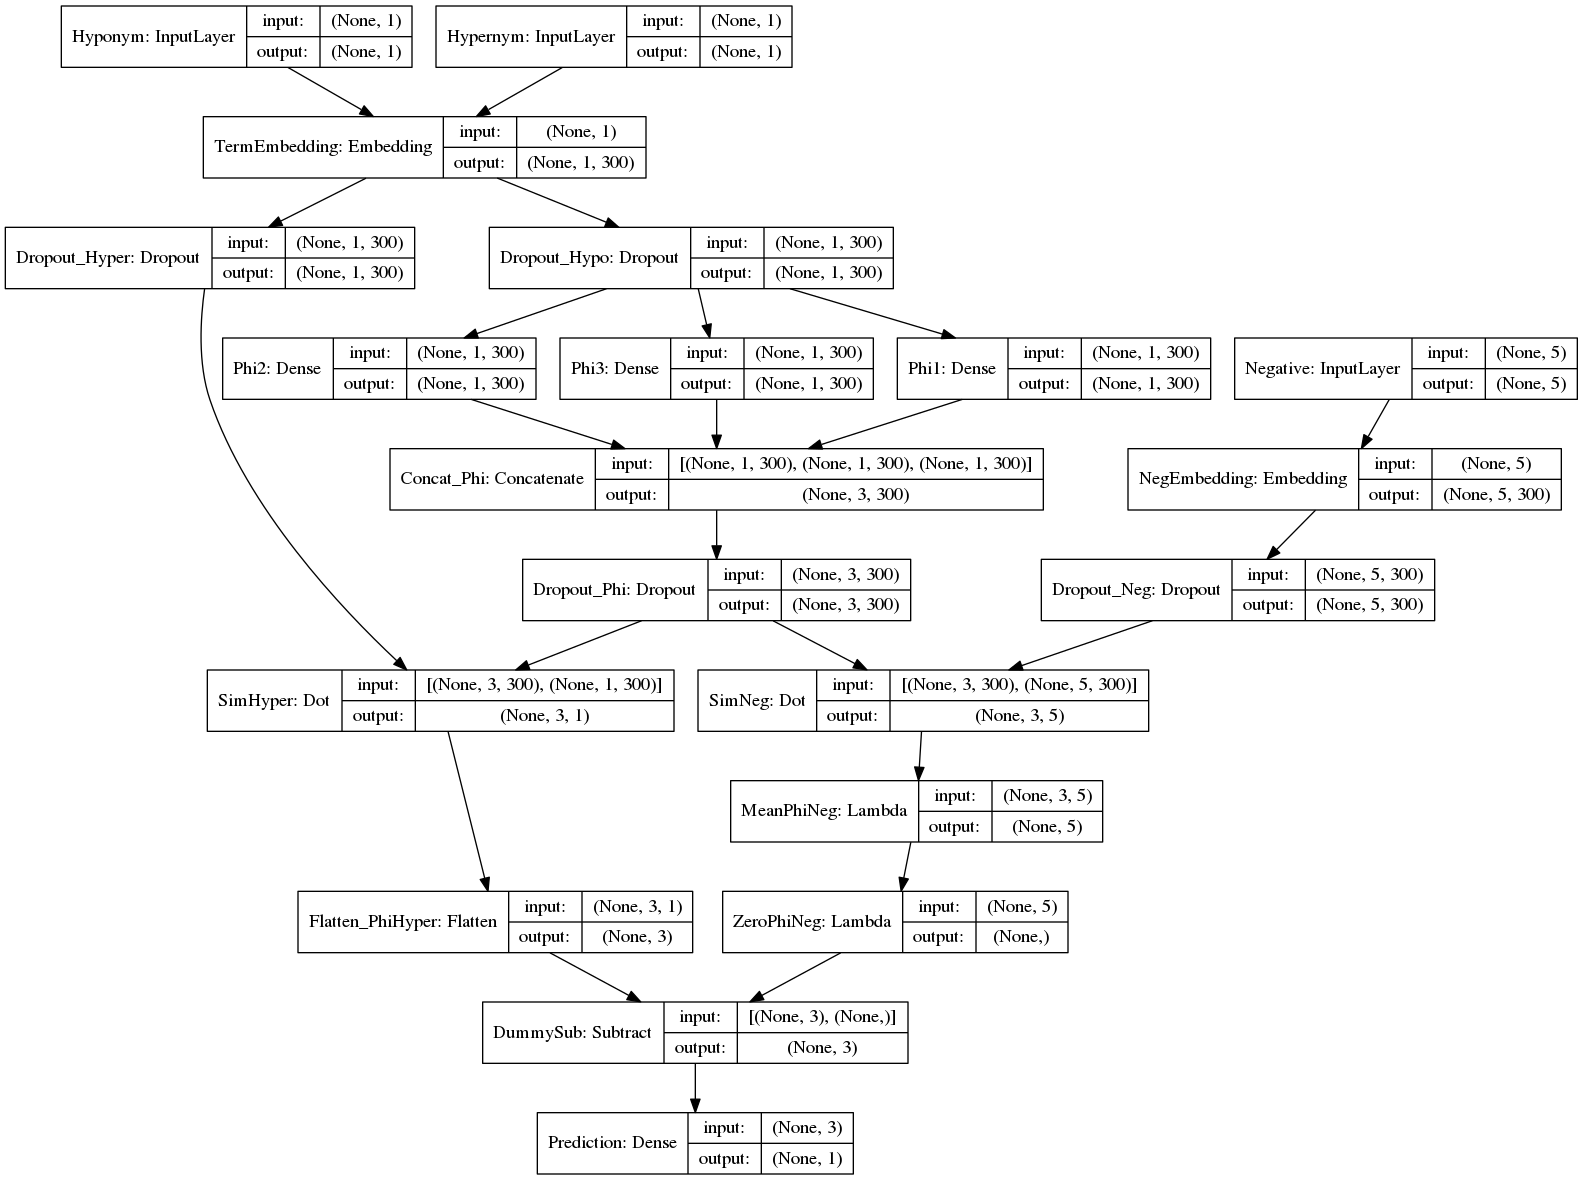
\includegraphics[width=1.\linewidth]{images/CRIM_multiphi_regularised.png}
  \caption{Multi-projection model schema}
  \label{fig:multiphi_model}
\end{figure}
A schema of our CRIM model implementation is illustrated in Figure~\ref{fig:multiphi_model}.  For the sake of readability, we limit the projection layer count to three but we tested model variants having up to ten projections layers in our experiments.  In the description below we represent the number of projections by the term $k$; in the context of the diagram $k=3$.  This model features three inputs: a hyponym word ID, a hypernym word ID and an unordered sequence of five words which are semantically similar to the hyponym including the hyponym itself and a sample of four randomly selected synonyms.  The inputs are captured in the InputLayers \textbf{Hyponym}, \textbf{Hypernym} and \textbf{Negative} respectively.

The hyponym and hypernym inputs are passed to a shared Embedding layer, \textbf{TermEmbedding} which fetches the word vector as described in \cref{dataset_preproc}.  The negative input, consisting of a list of five token IDs, is fed to the \textbf{NegEmbedding} layer which expects an input of length 5.  Both Embedding layers are initialised with the same weights we gathered from the pre-trained embeddings space relevant to the experiment.  A Dropout layer is added to each respective Embedding layer - \textbf{Dropout\_Hypo}, \textbf{Dropout\_Hyper}, and \textbf{Dropout\_Neg}) - which randomly sets 30\% of the embeddings dimensions to 0 disrupting none-generalisable patterns in the training data which may incline a model to over-fit.  The dropout rate was chosen arbitrarily, based on the recommendation in the Keras documentation; the actual dropout rate was not specified in the original paper \citep{bernier2018crim} but in the code they later published on GitHub, a default of 0.5 was suggested.

The fully-connected Dense layers \textbf{Phi1, Phi2, Phi3, $\ldots$} are responsible for learning aspects of the hypernymy transformation.  Constrained by space, we limit the model in Figure~\ref{fig:multiphi_model} to  three projection layers.  Since the model is expected to learn a linear projection transformation, we disable non-linear activation in these layers, reducing the model to combine the input hyponym embedding with the weights in each respective fully-connected dense layer.  The Dense layer's weights are contained in a 2D square matrix where each axis has dimensions equal to the embeddings vector.  Our pre-trained embeddings are all 300-dimensional; therefore, each projection matrix is $\bm{\Phi}_i \in \mathbb{R}^{300 \times 300}$, where $i \in \{1,\ldots,k\}$\footnote{$k=3$ in the diagram}, with a total of 90,000 trainable parameters per projection Dense layer.  We also eliminated the bias term from these layers since they do not form part of the technical specification.  The Dense layer weights are initialised with a custom-built initialiser which multiplies an identity matrix to a matrix populated with numbers drawn from a normal distribution with parameters $\mu=0$ and $\sigma=0.01$.  In their original paper \citet{bernier2018crim} \textit{add} the identity matrix to the array of random numbers but we observed slightly better results with this approach.

Each Dense layer outputs an estimated hypernym tensor which we combine into a unified projection matrix via the Concatenation layer \textbf{Concat\_Phi}, which is only responsible for merging the projection tensors and does not learn any parameters.  This operation yields a tensor $\bm{P} \in \mathbb{R}^{k\times300}$.  Dropout of 30\% is once again applied after the Concatenation layer.  The next step is to determine the similarity between each estimated hypernym projection and the positive or negative hypernym embedding derived from the input data.  Recall that we normalised our embeddings before commencing training; moreover, we set the \texttt{normalized} parameter of the Dot Merge layer \textbf{SimHyper} which ensures that the dot product is computed on unit-normalised embeddings and projections, thus yielding a score equivalent to cosine similarity.  Once the model is exposed to some training examples we expect the model to assign a relatively high similarity score to projections which have detected signals analogous to hypernymy and, conversely, a lower score to projections which learn parameters that run counter to hypernymy.  \textbf{SimHyper} outputs a 2D tensor consisting of single row of $k$ similarities, where $k$ is equal to the number of projections. This tensor is subsequently flattened by the layer \textbf{Flatten\_PhiHyper} to a column vector $\bm{s} \in \mathbb{R}^{k\times1}$.

We momentarily deviate from \citeauthor{bernier2018crim}'s published model by using a similar mechanism to measure the similarity between the projections and a matrix consisting of the  five negative input embeddings, which we formally refer to as $\bm{Z} \in \mathbb{R}^{300\times5}$.  \textbf{SimNeg} computes this transformation resulting in a 2D tensor $\bm{P}\cdot\bm{Z} = \bm{N} \in \mathbb{R}^{k\times5}$ which features the cosine similarity of every semantically-similar word with every estimated hypernym projection.  We reduce this tensor to $\bm{\bar{n}} \in \mathbb{R}^{5\times1}$, which denotes the vector of column means of $\bm{N}$. The operation is handled by the lambda layer \textbf{MeanPhiNeg}. We follow \citep{ustalov2017negative} and introduce asymmetric and neighbour regularisation with no re-projection, by computing the mean squared similarity, denoted $r$, between the non-hypernym, semantically-related words and the projected hypernym:
\[ r = \lambda \bigg( \frac{1}{\vert \bm{\bar{n}} \vert}\sum_{i=1}^{5} \bm{\bar{n}}_i^2 \bigg)\]
We created a customised loss function which adds the regularisation term $r$ to the standard binary cross entropy loss.  A hyperparameter weight $\lambda$ controls the influence of this regularisation term on the model's loss.  If the model projects hypernym vectors similar to a term's synonym or back to the term itself, a higher regularisation penalty will be excised, and vice versa.

Note that the negative input sequence is used for regularisation and is quite separate from the actual negative samples which are uniformly sampled from the vocabulary accompanied by a ground-truth $y=0$ value.  By employing this technique, we dissuade the model from projecting hypernyms which are too similar to the query term and the query term's synonyms while simultaneously also providing the model with random unrelated words as explicit example of non-hypernymy.  This should encourage the model to assign a low prediction score to random words which should make them ineligible as candidate terms when generating hypernyms for unseen test words.

We do not want the negative, similar word features to propagate to the model's classification head; at the same time we need to ensure that negative synonym operations are connected to the output or the Keras compiler will not acknowledge these component layers.  To solve this, we created a zero-valued, single- element vector by multiplying the mean of $\bm{\bar{n}}$ with 0 which we then subtract from our vector $\bm{s}$, effectively connecting the layers whilst making sure that they will not influence the affine layer parameters learned by the model's logistic regression classification \textit{head}.  These tensor operations are handled by \textbf{ZeroPhiNeg} and \textbf{DummySub} respectively.  The vector $\bm{s}$ containing the similarity values between each projection and candidate (positive or negative) hypernym passed to the training function is fed into the logistic classifier which learns $k$ feature parameters ($k$=number of projections) and a bias term.

Finally, we optimise gradient descent with the Adam algorithm \citep{kingma2014adam}, using the recommended parameters in the paper which includes the default learning rate of 0.001.  We underline that the original CRIM setup is not identical to ours.  \citet{bernier2018crim} tweak the $\beta_2$ value to 0.9 (from the original 0.999) and lower the learning rate by an order of magnitude.  Moreover, they only allow very small ($\pm0.0001$) gradients to propagate to the network.  They counter the effect of a very small learning rate and gradient clipping by training their model for several hundred epochs.  

Rather than gradient clipping, we incorporated gradient norm scaling whereby the gradients are scaled to a norm of 1 before being back-propagated to the network.  This should limit large gradient deltas during first training phases, although in our case, the effect would be less pronounced since the embeddings' weights are frozen.  These changes to the training algorithm allow us to reduce the training epoch remarkably, settling on 15.     

In the next sections, we describe the custom algorithm we built with which to train the model.

\subsubsection{CRIM Training Algorithm} \label{crim_training}
\begin{table*}\centering
    \begin{tabular}{@{}clllc@{}} \toprule
    \textbf{Batch Id} & \multicolumn{3}{c}{\textbf{Input X}} & \textbf{y} \\ \midrule
    & \textbf{Hypo.} & \textbf{Semantically Similar} & \textbf{Hyper.} &  \\ 
    %\cmidrule{2-4}
    \multirow{4}{*}{1} & rifle & \textit{dagger, pike, Kalashnikov, bazooka, rifle} & arm & \textbf{1}\\
    & rifle	& \textit{sword, shotgun, pistol, grenade, rifle} & Cleantech\_Investor & \textbf{0}\\
    & rifle & \textit{missile, spear, shotgun, hatchet, rifle} & E2D\_deals & \textbf{0}\\
    & rifle & \textit{kalashnikov, knife, sword, cannon, rifle} & corks\_popped & \textbf{0}\\ \midrule
    \multirow{4}{*}{2} & rice & \textit{rice, rice, rice, rice, rice} & grain & \textbf{1}\\
    & rice & \textit{rice, rice, rice, rice, rice} & Gentges & \textbf{0}\\
    & rice & \textit{rice, rice, rice, rice, rice} & Adumuah & \textbf{0}\\
    & rice & \textit{rice, rice, rice, rice, rice} & flannelette & \textbf{0}\\ \midrule
    \multirow{4}{*}{3} & gorilla & \textit{dog, cat, coyote, elephant, gorilla} & chordate & \textbf{1}\\
    & gorilla & \textit{cat, lion, dog, bull, gorilla} & chief\_Tariq\_Jamil & \textbf{0}\\
    & gorilla & \textit{lion, horse, goat, pig, gorilla} & Skevington & \textbf{0}\\
    & gorilla & \textit{sheep, rabbit, cow, bonobo, gorilla} & Heath\_Hocking & \textbf{0}\\
    \bottomrule
    \end{tabular}
    \caption{Example of augmented mini-batch featuring positive and negative hypernymy examples}\label{tab:mini_batch_example}
\end{table*}
Our training dataset is composed entirely of positive samples.  However, our model requires negative samples: both semantically-related and random.  We could have added synthetic, negative examples to the training set according to a specific ratio (e.g. 10 negative examples for every 1 positive).  However, this approach limits the negative vocabulary diversity the model is exposed to since it will see the same negative examples in every epoch.  Also, batches are sampled randomly and, although the distribution of positive to negative examples should tally with the overall distribution in the dataset, it is unlikely that positive and negative examples of the same query term are drawn in the same mini-batch sample. 

Instead, we customised the training algorithm such that: negative samples are uniformly sampled from the vocabulary during the training phase; negative and positive hypernyms of the randomly-drawn query terms feature in the same mini-batch.  The training fold was shuffled before every epoch and 32 positive examples sampled for every batch update, with each example augmented as follows.  Negative hypernym words are dynamically sampled in the way we described at different ratios (1, 5, and 10 for every positive sample).  The negative examples will feature in the $hyper$-slot of the $(hypo,hyper)$ word-pair such that $1+m$ rows are generated for every positive word-pair, where $m$ is the negative sample count.  Therefore, given a positive-to-negative ratio of 1:10, a 32-positive-sample batch will be augmented to a 352-mixed sample batch.  Since projection learning is a supervised learning technique, we need to accompany each pair with a $\bm{y}$ value, where 1 represents positive hypernymy, and 0 indicates the absence of the semantic relationship.

In the same phase, we also select words that are semantically linked to the query term but are not hypernyms and use these words to regularise a customised loss function as described in \cref{multi-proj-model}.  We opt for five such words, of which one is is the query word itself.  Some query words are linked to more than four synonyms in the dataset; in that case we randomly choose four from the available synonyms.  Other words have less than four synonyms available in which case we default the rest of the words to the query term.  If all five words are set to the query term, then the regularisation term $r$ (refer to \cref{multi-proj-model}) is reduced to the average cosine similarity between the query term and each projection.  A small excerpt of a mini-batch consisting of three positive word-pairs augmented by three negative samples is illustrated in Table~\ref{tab:mini_batch_example}.  We are showing the words in the table for the sake of clarity but recall that the training set words are converted to token IDs before being fed to the model.

We increment the training loss for every batch gradient update, finally dividing it by the total number of updates to get the mean epoch training loss.  We measure the test loss in a similar manner, also augmenting test positive samples by the same number of negative samples we used during training.  In this way, we maintain the same distribution of positive to negative samples in both training and test folds for every epoch.  The test loss is not necessarily a predictor of the quality of the generated hypernyms.  The MAP, MRR and P$@k$ metrics measure the correctness of discovered hypernyms more accurately.  

\subsubsection{Grid-search for Optimal Hyperparameters}
Our objective is to explore the model hyperparameters which yield the best performance on our standard, combined dataset.  Our model selection process is based on four dimensions: the embedding vector space (word2vec, GloVe, fastText); the number of $k$ projections (1, 5, 10); the negative sample count (1, 5, 10); and the combined asymmetric and neighbour regularisation strength parameter $\lambda$ (0, 0.1, 1.0).  In this set of experiments we do not employ early stopping and train each model for exactly 15 epochs.  

We cross-validate each model on 5 folds, fitting a total of 405 models.  Once again, we evaluate performance based on the SemEval-2018, Task 9 metrics, running the same modified scorer we employed in the previous round of experiments.  Besides being able to determine which feature yields statistically significant performance increases, we will also be able to compare the multi-projection results with those produced by the \ac{MSE}-based hard-clustering experiments we described in \cref{ustalov_experiment}.  

\subsubsection{CRIM Prediction Algorithm} \label{crim_prediction}
Binary cross-entropy models recast hypernym discovery as a classification problem.  Generating hypernyms for a given query term involves running the network's forward propagation for every candidate term in a vocabulary.  Each time, the network will output a probability - based on the pre-trained embeddings weights and the trained weights in the projection layer and logistic regression layer - of the candidate word being a suitable hypernym of the given query term.  Assuming a vocabulary of 250,000 words and a test set of 400 queries, this means 100 million forward propagations to evaluate a relatively small test set once.  Our model features the additional complexity of computing the similarity between the projections and the synonymous input words which, as we explained in \cref{crim_model_structure}, does not directly contribute to the output probability.  Lastly, we are not really interested in the hypernymy probability \textit{per se}; we merely need some scalar value with which to rank our words.

To side-step these issues, we devised a simple mechanism which leverages fast \texttt{numpy} matrix operations to execute the same operations performed by the neural model.  We extract the weights from the network and load the embeddings, projection transformations and classifier weights to \texttt{numpy} arrays.  The projection matrices are loaded into a 3D matrix which allows us to estimate $k$ hypernyms in a single operation by applying the dot-product on the 3D matrix and the term query embeddings vector.  In a second operation we compute the similarity of every vector in the embeddings space with every projected hypernym and apply the logistic regression parameters to the linear combination of similarities and bias term.  We are able to do this by exploiting \texttt{numpy}'s broadcasting feature which saves us from running expensive loops in native Python.  

We forfeit feeding the result of the linear combination to the sigmoid function since the sigmoid function usually grows monotonically and we are only interested in ranking words based on descending scores.  The process is repeated for every word in the test set, producing a dictionary where the key is the query term and an ordered list of hypernyms is the value.  We evaluate the results using the SemEval-2018 Task 9 scorer, slightly modified to read the results from the aforementioned dictionary.

\subsection{Joint-Learning of Clusters and Projection Parameters (Yamane)}
This model, the original of which we reviewed in \cref{yamane_in_review}, is the ancestor of the CRIM.  Developed by \citet{yamane2016distributional}, it is also based on the binary cross-entropy objective function and also extracts cosine similarity features, given hyponym and hypernym embeddings.  It is distinguished by the training algorithm which learns several models, each model representing a cluster, and training samples allocated to the model which returns the highest similarity score for an input word-pair.  Each model learns a projection matrix and bias term parameters.

\citet{yamane2016distributional} claimed the model delivered superior results to \ac{MSE}-based hard-clustered solutions but tested the models on a single English dataset and did not report statistical significance.  Our objective in this experiment is to analyse the model's performance with respect to the "pipeline" models which cluster the dataset prior to training, using the same combined dataset and evaluation metrics we have employed so far.  We are also curious to see whether the multi-projection novelty is superior to the original algorithm which inspired it.  Finally, we will evaluate the Yamane model on several pre-trained embeddings as we have done with the preceding models.  

The paper's authors never released the model's source code since the intellectual property belongs to the Toyota corporation.  We followed the paper and built the model ourselves, using the Keras machine learning framework.  We describe the model and training algorithm in the following sections.  For the sake of brevity, we may refer to the joint model as \textbf{Yamane}.

\subsubsection{Yamane Model Structure} \label{yamane_model_structure}
Yamane is an ensemble solution which creates and trains new clusters if a particular training pair scores below a set threshold ($\lambda$) on already-existing models.  Maintaining the ensemble introduces complexity in the training algorithm, but each cluster in the model behaves in exactly the same manner.  

Indeed, the structure of a single cluster is fundamentally a simplified version of the multi-projection model, due to the former's reliance on only a single fully-connected layer assigned to learn the projection matrix.  Thus, the cluster extracts a single similarity feature, computed by applying the dot-product operation on the projected hypernym vector and input (positive or negative) hypernym embeddings.  Furthermore, the cluster's logistic classifier \textit{head} does not learn a coefficient for the similarity score feature but only learns a bias term.  We do not embellish the structure by introducing a regularisation term, but adhere to the base implementation as presented in \citep{yamane2016distributional}.

The fully-connected layer consists of 300 nodes, same as the embeddings dimensionality, and is initialised with numbers drawn from the Glorot uniform distribution.  This is the default weight initialiser the Keras developers have assigned to the Dense layer and we use this because \citet{yamane2016distributional} do not mention a specific initialisation strategy.  The bias term in the logistic layer is initialised to 0.  The Dot operator, responsible for calculating the similarity between the projected hypernym and actual hypernym, normalised both inputs to unit-length such that the dot-product returns the cosine similarity of the two vectors.  The model is optimised with the Adam algorithm \citep{kingma2014adam} using the default parameters.  Unlike in the multi-projection model, we do not peruse of either dropout or gradient clipping since these steps are not included in the original paper's methodology.

Models which rely on large-vocabulary embeddings have a significant memory footprint.  A 250,000 vocabulary, each word represented by a 300-dimensional, 32-bit float vector will require approximately 286 MB of memory.  Depending on the dataset size and hyperparameter $\lambda$, joint ensembles can create a multitude of clusters;  \citep{yamane2016distributional} report up to 44 for a particular experiment setup.
A conservative ensemble composed of 10 cluster would require approximately 2.7 GB of memory.  Our experiments often require the creation of several hundred models within a Jupyter environment (depending on how many hyperparameters we are exploring); such memory requirements are expensive to address.

Keras supports the concept of using models as layers in other models.  We exploited this feature to create an embeddings-lookup standalone model which simply returns the hyponym and hypernym embeddings corresponding to the input word-pair.  This model is not compiled because it does not feature an objective function and does not need to be optimised for gradient descent. We shall refer to this as the \textit{Embeddings Model}.  This model is referenced as the embeddings layer for every new cluster we create.  The cluster word-pair inputs are wired to the \textit{Embeddings Model} and the hyponym and hypernym embeddings outputs are connected to the fully-connected layer and dot-product similarity layer respectively.

The advantage is that we are reusing the same embeddings layer reference in every new cluster created when training the ensemble.  The weights of the embeddings in \textit{Embeddings Model} are frozen so they are impervious to the gradient when back-propagating a cluster's error.  The embeddings weights are only allocated once, when the \textit{Embeddings Model} is first created.  Besides limiting memory consumption, this technique reduces the time required to create and compile each new cluster.

\subsubsection{Yamane Training Algorithm}
Before commencing training, we initialise the ensemble with a single cluster, following the details we mentioned in \cref{yamane_model_structure}.  As in the multi-projection case, the dataset is composed entirely of positive hypernym samples.  The training fold is shuffled at the beginning of every epoch.  The batch size needs to be reduced to a single example because every sample has to be evaluated against all clusters before being assigned to a specific one.  We invoke the prediction method of every cluster on this example to determine the cluster to which we will assign the sample.  The cluster which returns the highest prediction probability according to its current weights, "wins" the word-pair and its parameters are trained on that sample.  If the highest prediction is lower than a set threshold (the hyperparameter $\lambda$ ), then a new cluster is created and the sample automatically assigned to it.

Once the sample is allocated to an existing or new cluster, the single-sample is augmented by negative examples which are randomly selected from the embeddings vocabulary in the same manner described in \cref{crim_training}.  However, we do not sample synonyms for regularisation in this case.  The number of negative samples is configurable.

Loss is accumulated on every cluster and we report the training loss at the end of every epoch by calculating the mean loss across all the clusters in the ensemble.  Instead of reporting validation loss, we calculate \ac{MRR} and \ac{MAP} on the validation fold which are our target metrics.  We do this because we observe that loss and \ac{MRR}/\ac{MAP} are not correlated.  Calculating the evaluation metrics on the validation fold increases the algorithm's training cost even further since hypernym prediction - as explained in \cref{yamane_prediction} below - is particularly expensive with this model.  For every query word we need to first compute the hypernym prediction for every word in the embeddings space according to each cluster.  The more clusters are created, the slower training and evaluation become.

From preliminary experiments, we found these models challenging to train.  In the context of single set of hyperparameters, the experience sometimes changed remarkably from one training fold to the other.  There was a general tendency for the most recent clusters to win samples which had contributed to the training of older clusters for several epochs.  We implemented early stopping to mitigate this problem.  We maintained the best validation MAP result observed in a particular training cycle and compared each epoch's MAP to the best score.  Whenever a better result was found, we updated the best score and persisted the clusters' projection and bias parameters to disc.  However, we disabled early stopping for the first three epochs since the model could be unstable during the initial training cycles.  We avoided saving the embeddings weights as well because: i) they do not change during the training process and thus can be easily re-loaded from memory; ii) we wanted to keep the weight array as small as possible to speed up both saving and loading the weights back to the model. If the score failed to improve for two epochs, we stop the training process outright and reload the best performing model before performing an evaluation on the validation test.  This parameter is referred to as \textit{patience} and we implemented it as a configurable parameter.

\subsubsection{Experiment Setup}
Once again we perform 5-fold cross-validation on the combined English dataset employed in \citep{ustalov2017negative} consisting of \textit{BLESS} \citep{Baroni2011}, \textit{EVALution} \citep{santus2015evalution}, \textit{ROOT09} \citep{santus2016nine}, and \textit{K\&H+N} \citep{necsulescu2015reading}, the same we have used in all our experiments so far.

In this set of experiments, we do not embark on a costly grid-search for the optimal hyperparameters.  Training of the Yamane algorithm is very slow since every word-pair in the training set must undergo two phases: evaluated against all clusters to see which yields the highest hypernymy probability; the actual training of the assigned cluster's parameters.  Moreover, the original experiments suggest that the algorithm does not create effective clusters in an English context \citep{yamane2016distributional}.  

Our aim is to find parameters which trigger the creation of a small number of clusters, in the range of 2 to 10 which offers a good balance of enough clusters to capture our data's diversity but not too many as to make training too slow.  We performed preliminary experiments on a small subset of the dataset and observed how many clusters were being created at every epoch, whether cluster stability is reached and the performance impact on an unseen validation set.  These element are influenced by the choice of embeddings, number of negative samples, and the $\lambda$ threshold parameter, the latter hyperparameter having the strongest effect on cluster creation.

We initially experiment with 1, 5 and 10 negative samples.  We found that a single negative sample does not encourage the model to create new clusters, so the joint element in the training is lost.  Increasing the negative samples to 5 caused the model to create new cluster when training on all embeddings types, while 10 negative samples were found to have a slight negative effect.  We therefore opted to train our Yamane implementation on 5 negative samples.

The $\lambda$ threshold parameters is very sensitive.  Changing it by a single point can cause the model to create several new clusters at every epoch, with each created cluster taking its toll on both training and post-epoch evaluation times.  We finally settled on 0.16 for word2vec and GloVe embeddings while opting for 0.18 in the case of fastText embeddings.

We train for a maximum of 10 epochs, although the training cycle may be terminated by the early stopping logic we executed after every epoch.

\subsubsection{Yamane Prediction Algorithm} \label{yamane_prediction}
The ensemble model also frames hypernym discovery as a classification problem.  Generating hypernyms is more complex than in the multi-projection model case because we have to contend with multiple models.  For a given test query, we need to compute the 
hypernym probability of every word in the vocabulary.  In \cref{crim_prediction}, we noted that a 400-word validation set and a 250,000-word vocabulary results in running the model's forward propagation 100 million times.  The number increases 10 times' fold if we have a 10-cluster ensemble by the end of the training phase.  

We implemented a similar algorithm as presented in \cref{crim_prediction}.  We extracted the projection matrix and bias weight from every cluster and loaded them in a 3D \texttt{numpy} matrix and column vector respectively.  By applying the dot product of the combined projection matrix and the embeddings of a given query term, we immediately compute $k$ hypernym projections, where $k$ is the number of clusters in the ensemble.  We normalise each projection to unit-length before combining the normalised projection matrix to a matrix of all the vocabulary embeddings.  This yields a matrix of cosine similarity values, where each row represents a vocabulary word and each column the cosine similarity of that word with a projected hypernym generated by each respective cluster.

We find the maximum projected cosine similarity value for every vocabulary word, by finding the maximum value along the second axis, ending with a column vector where an element at index $i$ corresponds to the final similarity of the word $i$ with the query term's projected hypernym.  Finally, we perform an \texttt{argsort} on the column vector which effectively indicates the index of the word whose vector is closest to the projected hypernym.  We emit the 15 closest words as our hypernym predictions for a given query term.

\subsection{Computational Setup}
No dependencies were fundamentally changed from the setup we described in \cref{computational_setup_orig}.  The main deviation from that previous crop of experiments, is the use of Keras to build the neural learning models.  However, Keras is shipped with TensorFlow so a separate installation was not necessary.  The binary cross-entropy models required more computational power due to a more complex model and training algorithm.  We moved our EC2 instance to more powerful hardware, the \textit{c5.2xlarge} platform which is optimised for heavier CPU usage.


%% mention AWS EC2 setup
%% jupyter-scipy docker, based on a Python 3.6 environment to avoid installing dependencies
%% Upgraded dependencies from Ustalov's original experiment.

\section{Experiments on Shared Task Corpus and Data}
The hypernym discovery dataset as outlined in the shared task \citep{camacho2018semeval}, is substantially different to the combined dataset with which we worked in our initial experiment batch:
\begin{itemize}
    \item Besides single words, bi-grams and tri-grams are also featured;
    \item The query terms are distinguished between common terms and entities (proper nouns);
    \item While the combined dataset we used in our first batch of experiments was particularly focused on biology\footnote{31\% of all words are mapped to the following semantically-related hypernyms: \textit{animal, plant, chordate, vertebrate, mammal, placental, herb, invertebrate}.}, the shared task dataset features words which are more varied in domain: 5,599 distinct hypernyms across the training, test and validation data splits;
    \item Word senses are conflated.  Hypernyms are given for all senses of a given word.  For instance the gold-standard hypernyms for the query word \textit{fault} include \textit{fissure} and \textit{imperfection} which capture the geological and failure senses of the lexicalisation;
    \item Despite the two-step hypernym validation process, the dataset is noisy whereby the gold standard pairs are not necessarily correct\footnote{This was also confirmed by the shared task's organisers in private correspondence.}.  For instance, the given hypernyms for \textit{Campo San Polo} (Venetian square) include \textit{topological manifold} and \textit{hausdorff space} which are two mathematical concepts that are unrelated to the single \textit{public square} sense of the word.  Models will therefore have to confront positive training pairs which will actually penalise their performance.
\end{itemize}

For the general-purpose English shared task, the authors deviated from the popular Wikipedia dump, which powered so many \ac{VSM}s in the literature.  They opted instead for the \textit{UMBC} corpus \citep{han2013umbc_ebiquity} which is not encyclopedic in nature, being composed of paragraphs originating from diverse web sources.  Therefore, we could no longer rely on the readily available pre-trained embeddings we used in the first batch of experiments. Instead, we trained our embedding on the given corpus after processing it to merge tri-grams and bi-grams such that these multi-word tokens are treated as single words in the embeddings vocabulary.  

In our initial experiment run, we tried out all the reviewed projection learning algorithms.  After careful evaluation of each model in terms of performance and training complexity, we opted to use exclusively the CRIM model.  %Our implementation - although underpinned by the same mathematical principles as the original - had different 

Furthermore, we extended our initial, basic implementation of CRIM in the following ways:
\begin{enumerate}
    \item Following \citep{bernier2018crim}, we implemented the hard parameter sharing flavour of multi-task learning \citep{ruder2017overview} whereby we trained two classifiers on concepts and entities respectively, each sharing a common feature extraction layer;
    \item We found that, despite training for only 15-20 epochs, the models converged quickly. To avoid "over-shooting" the best possible result, we integrated early stopping to our custom training algorithm and serialised the weights of the best-performing model during training;
    \item We fine-tuned the embeddings in a second phase, by first learning the projection matrices on fixed embeddings features, and after convergence, froze the projection matrices and trained the embeddings for a few more epochs until no performance increase was detected on the validation set.
\end{enumerate}

Finally, we experimented with word features extracted from our custom word2vec, GloVe and fastText embeddings trained on the \textit{UMBC} corpus.  

\subsection{Preprocessing the Corpus} \label{semeval_preprocessing}
The \textit{UMBC} corpus was available in two formats: raw and pre-tokenised.  In the latter version, the raw text had been tokenised and parsed with every sentence featuring in its own line.  The corpus was made up of approximately 132.5 million lines and 3 billion words. 

The vocabulary size, including candidate and dataset words, is $219,682$ words.  Of these, $160,798$ are unigrams; $52,121$ are bi-grams; $6,763$ are tri-grams.  Unless the corpus is first processed with a phrase matcher, only embeddings for single words will be learned.  It was possible to create bi-grams and tri-grams from the corpus text, but that would means learning bi-gram and tri-gram embeddings exclusively.  This would have resulted in a very sparse context since bi-gram and tri-gram target words are in general rarer than the single words of which they are composed (e.g. \textit{fast red car} will be less frequent than simply \textit{car}).  

Instead, we used the provided vocabulary to merge bi-gram and tri-grams in an atomic token, replacing the space delimiter with the underscore character.  To carry out this task, we executed a pre-processing script which Gabriel Bernier-Colborne published on GitHub \footnote{\url{https://github.com/gbcolborne/hypernym_discovery/blob/master/prep_corpus.py}}.  The script required the pre-tokenised corpus since it expected one sentence per line.  It was able to scale gracefully, by looping over the file, loading one line into a memory at a time.  The script performed a first pass on the corpus file to create an $n-$gram frequency dictionary ($n \leq 3$), given that the $n-$gram was present in the provided vocabulary file. The script then iterated once more on every sentence/line in the file, extracting every $n-gram$ in a sentence, resolving overlap conflicts by using the frequency dictionary to prioritise lower-frequency multi-word terms.  Finally, Bernier-Colborne's script collapsed the multi-word spans into a single token by substituting the delimiting spaces with an underscore.  The line was appended to a new text file.  Prior to exiting, the script counted the frequency of the unified tri-grams, bi-grams, and unigrams and emitted the histogram together with the processed corpus.  Contrary to what was stated in \citep{camacho2018semeval}, 159 words in the provided vocabulary did not feature at all in the corpus.

We executed the script on \textbf{Dante}, the University of Malta's Department of Physics, Institute of Space Sciences and Astronomy (ISSA) HPC GPU cluster.  A serial \texttt{slurm} job was submitted to the cluster's head node, requesting a single node.  The preprocessing job was completed in around 5 hours.

\subsection{Training Word Embeddings}
\begin{table*}\centering
    \begin{tabular}{@{}lrrrr@{}} \toprule
    & \textbf{Dimension} & \textbf{Epochs} & \textbf{Window Size} & \textbf{Negative Samples} \\ \cmidrule{2-5}
    \textbf{word2vec} & 300 & 10 & 8 & 10 \\  
    \textbf{fastText} & 300 & 15 & 8 & 5 \\
    \textbf{GloVe} & 300 & 25 & 15 & - \\
    \bottomrule
    \end{tabular}
    \caption{Embeddings systems' main hyperparameters.}\label{tab:semeval_embeddings_hyper}
\end{table*}
We wanted to evaluate our models on word2vec, GloVe and fastText embeddings.  We downloaded a fast \texttt{C++} implementation of each embeddings model and compiled the code by invoking the \texttt{make} command.  Each embeddings model expects a set of hyperparameters which controls the various aspects of the algorithm.  In most cases, we retained the default parameter values set by the models' original designers and which ostensibly should generate embeddings suitable for most tasks.  We tuned a small number of parameters as reflected in Table~\ref{tab:semeval_embeddings_hyper}.  Common to all embeddings is the dimensionality: we opted for 300-dimensional vectors throughout since we assumed our corpus is large enough to sustain such a number of latent features.

word2vec and fastText learn embeddings via a similar mechanism, the main distinction being that fastText exploits character n-grams to learn representations for subwords along with the word itself.  Both algorithms support two language model objectives: \ac{CBOW} and skip-gram.  In either case, we selected the skip-gram objective which predicts context words around a target word.  Skip-gram is believed to generate embeddings that perform better at semantic tasks \citep{mikolov2013distributed} but requires a larger dataset to learn the nuances of similar words.  We believe this prerequisite is satisfied by our 3-billion word corpus.  

We used negative sampling loss for both word2vec and fastText.  The recommended number of negative samples is normally in the range $[3-10]$ and we arbitrarily choose 10 and 5 for word2vec and fastText respectively.  We selected a context window of 8 words for both embeddings models which we considered a  reasonable trade-off between grabbing sufficient context around each word in a sentence and the model's ultimate complexity.  We set the sampling threshold to $1\times10^{-5}$ which reduces the probability of sampling highly frequent, and hence uninformative, words.  We experimented with different training cycles, training word2vec and fastText for 10 and 15 epochs respectively.  We kept the default learning rate for word2vec (0.025 in case of skip-gram) but increased the learning rate to 0.1 for fastText training.  

The word2vec algorithm accepts a vocabulary file and we specified the histogram file output by the preprocessing script we described in \cref{semeval_preprocessing}.  This ensured that embeddings would only be generated for words in the given vocabulary, the only exception being 159 words which were in the vocabulary but which were somehow not found in the corpus proper.  We could not specify a vocabulary parameter for the fastText trainer; instead we set a minimum occurrence count of 5 words, which was the minimum threshold set by the shared task's organisers for a word to be included in a general-purpose vocabulary \citep{camacho2018semeval}.  
GloVe employs a different mechanism altogether, which aims to derive meaning from the co-occurrence probability ratio of two words.  Generating GloVe embeddings involved executing four scripts:
\begin{enumerate}
    \item Given a tokenised corpus, the first script \texttt{vocab\_count} creates a vocabulary allowing the user to specify limits such as a minimum frequency count.  We could forfeit this step, because the corpus pre-processing step emitted a word histogram along with the modified corpus;
    \item Given a vocabulary file, \texttt{cooccur} creates a co-occurrence matrix.  We resorted to default parameters which included a context window size of 15 words;
    \item Unsurprisingly, \texttt{shuffle} randomises the order of the words in the original co-occurrence matrix generated by the previous script;
    \item Finally, the \texttt{glove} script trains the GloVe embeddings on the supplied shuffled co-occurrence file and vocabulary file.  We trained GloVe for a maximum of 25 iterations.  
\end{enumerate}

Our hyperparameter selection approach could have been more exhaustive, generating a great deal of embeddings from a range of hyperparameters and evaluating each variant accordingly.  However, this would have required far more time and our objective was to study the effect of different embeddings models rather than the effect of various hyperparameters on a single model.  Our initial experiments already provided us with an inkling of which embeddings were likely - based on our previous results - to perform better on the hypernym discovery task, irrespective of the embeddings creation parameters.

We trained embeddings on \textbf{Dante} this time exploiting the multi-threading capability of the original \texttt{C++} implementation of the respective three algorithms.  We submitted \texttt{slurm} jobs requesting 8 nodes to train word2vec embeddings and 16 nodes to train GloVe and fastText embeddings respectively.  At around 4 hours, GloVe embeddings were the fastest to train, with most of the processing time dedicated to computing the word co-occurrence matrix.  48 hours were required to train fastText embeddings over 15 epochs while word2vec was trained for 10 epochs requiring 18 hours of computation time.  Jobs were submitted serially, waiting for one to complete before submitting another job.  

\subsection{Training Basic CRIM}
We described the CRIM model structure and training algorithm in \cref{crim_model_structure} and \cref{crim_training} respectively.  In the first round of experiments on the shared task dataset, we trained a CRIM model on concepts and entities separately, and on the full training set.  Each trained model was subsequently validated on:
\begin{itemize}
    \item Concept query words, exclusively;
    \item Entity query words, exclusively;
    \item All words in the test set (i.e. concepts + entities);
\end{itemize}
Contrary to our previous experiments, we do not create our own random data splits but stick to the training, test and validation sets provided by the shared task's authors.

The CRIM model in this case differs from the version we employed in the previous round of experiments, by an early stopping function we integrated in the training algorithm.  To determine how well (or badly) the model is learning the hypernym transformation, we compute the \ac{MAP} evaluation score on the given validation set after every completed epoch.  We keep track of the highest \ac{MAP} score we observe and stop the training cycle prematurely if \ac{MAP} does not improve on the current best result for three consecutive epochs.  To retain the best model, we serialise the weights to disc every time a new highest \ac{MAP} score is recorded.  We do not save the embeddings weights since we are using frozen pre-trained embeddings which are already available on disc.  

We also wanted to explore whether changing the number of internal projection layers would have an effect on the validation results.  We trained three models initialised with 1, 5 and 10 projection matrices respectively.  We eschew experimenting with the other hyperparameters and fix the negative sample count, dropout rate, and batch size to 10, 0.3, and 32 respectively.  Based on our first round of experiments, we found that these hyperparameters returned comparably very good results.  Gradient descent is optimised by Adam \citep{kingma2014adam} and we keep the optimiser's default parameters, except $\beta_2$ which we set to 0.9 following \citep{bernier2018crim}.  Each model is trained for a maximum of 15 epochs.

We investigate the effect of the word2vec, GloVe, and fastText word features by repeating each experiment three times, once for every embeddings space we trained on the \textit{UMBC} corpus dataset.  Once we are confident on having trained the best possible model, we load the best-performing weights from disc and  evaluate the model's actual performance by generating hypernym predictions for the query words in the held-out test set.  The shared task scorer is executed on the predictions and gold-standard hypernyms to calculate the ultimate \ac{MAP}, \ac{MRR} and P$@k$ scores.

\subsection{Multi-task Learning with CRIM}
\citet{bernier2018crim} tried a multi-task learning setup where they recast their model to learn hypernym projection for concepts and entities as two separate tasks which share the same embeddings, projection matrix and cosine similarity upstream features.  This \ac{MTL} strategy is known as hard parameter sharing and provides regularisation benefits to the model since the feature representation that is being learning needs to accommodate two (or more) objectives \citep{ruder2017overview}.

Gabriel Bernier-Colborne kindly clarified the \ac{MTL} setup details which were not included in the original paper due to lack of space.  We exploited Keras' \texttt{Functional} API which allows entire models to be reused as shared layers in other models.  We created a feature extractor model which learns $k$ projections (where $k \in \{1, 5, 10\}$  and outputs a vector of $k$ similarities as described in \cref{crim_model_structure}.  We do not compile this model since it will function as a shared layer within two logistic classifier models which learn the optimal similarity feature coefficients for concepts and embeddings respectively.

The training algorithm was modified as follows.  The model was trained on the full test set comprising both concepts and entities.  The training set is shuffled before every epoch so each batch will likely contain a mix of concept and entity hypernymy tuples.  We then separated concept and entity tuples into two homogeneous sub-batches, augment them with negative examples as explained in \cref{crim_training}, and feed them to the concept and entity logistic classifiers respectively.  The error from both the concept and entity objective functions is propagated to the common feature extractor layer/model thus modifying the projection weights which should improve hypernym prediction for both concept and entity terms.  We increased the batch size to 64 positive samples (from 32), considering that this batch will be split into two smaller batches prior to being fed to the respective classifiers.  To predict hypernyms, we need to apply either the concept or entity logistic regression parameters depending on whether the query term is a concept or entity respectively.  The projection matrix weights are common to all query terms irrespective of their type.

We setup our shared feature extractor with 1, 5 and 10 projection layers and train each variation on word2vec, GloVe and fastText embeddings.

\subsection{Transfer Learning with CRIM}
In our last experiment, we fine-tuned our pre-trained embeddings to suit the hypernym discovery task.  Training the embeddings with the rest of the network, may lead to obliterating the original weights and "forgetting" the word relationships due to large gradient fluctuations during the initial training epochs \citep{howard2018universal}.  This is exacerbated even if the training dataset is small.

To avoid this problem, we devised a strategy whereby we first trained the projection layer weights and logistic regression coefficients while keeping the embeddings frozen; the weights will not respond to gradient updates.  Let us refer to this as the \textit{base model}.  We stopped training, once the validation scores peaked, indicating that a good set of projection weights and logistic regression parameters were learned.  

We then initialised a new model, which was structurally identical to the base model, in terms of the supported number of projections (refer to Phi$k$ tensors in Figure~\ref{fig:multiphi_model}).  We will refer to the new model as \textit{transfer model}.  We set the weights of the transfer model's projection and logistic regression layers to the base model's trained weights.  The projection layer weights were then frozen to stop them from changing while we tuned the embeddings but we allowed the logistic regression parameters to be updated during training.  Conversely, the embeddings weights were set to trainable.  We set a unit-norm constraint on the embeddings weights second axis.  This ensured that each word vector in the embedding space remains normalised to make the dot-product which compares the hypernym projection with actual hypernym vector equivalent to cosine similarity (refer to SimHyper operation in Figure~\ref{fig:multiphi_model}).

We optimised gradient descent with Adam \citep{kingma2014adam} but reduced the learning rate by half to 0.0005.  The rate of the dropout layers after the embeddings and projection layers was increased from 0.3 to 0.5.  The updated model was trained in the same manner as described in \cref{crim_training}.  We attempted to tune the embeddings using two training datasets: concepts and entities; concepts only.  As we show in Chapter 4, \cref{dataset_stats}, the entities dataset contains a relatively high concentration of \textit{person} hypernyms.  This might induce the model to tune the embeddings to pull the \textit{person} vector close to several projections.  When focusing on concepts only, we roughly half the number of word-pairs where the hypernym is \textit{person}.

We impose more stringent early stopping parameters: we decrease the patience parameter to 1 which stops training once a single epoch yields a validation score which is less than the current maximum; we also reduce the maximum epochs to 5.  These precautions were intended to reduce over-fitting as much as possible.  We repeated the process for each of the three embeddings spaces to determine whether tuning improves the performance irrespective of the embeddings features.

\section{Summary}
We opened this chapter by describing our dual experimental objectives.  Inspired by a comprehensive analysis of unsupervised methods \citep{shwartz2017siege}, we first devised a common experimental setup against which to test the chosen four projection model variants. We extended the current research by: training the models on pre-trained GloVe and fastText embeddings in addition to word2vec features; applying statistical rigour to discover the extent that the models’ hyperparameters influence performance and which architecture yields statistically significant better results. 

In the second phase of our work, we chose the statistically best-performing model and applied it on the Shared Task-2018 Task 9, general-purpose, English subtask \citep{camacho2018semeval}.  We deviated from the original model \citep{bernier2018crim} in two ways: we evaluated it using features extracted from word2vec, GloVe and fastText embeddings; and we designed a two-phase training strategy inspired by transfer learning principles \citep{howard2018universal}, via which we were able to decrease considerably the training epochs.

We provided details of our implementation of the binary cross-entropy models, based on the technical description furnished in their respective papers \citep{yamane2016distributional, bernier2018crim}, using the \texttt{Keras} framework supplied with \texttt{TensorFlow}.  We had access to implementations of the mean square error models \citep{Fu2014, ustalov2017negative}, but we described how we tailored the code to fit our experimental regime.

Whilst we were able to train our models on publicly-available embeddings for the first tranche of experiments, our second set of experiments was distinguished by the fact that we trained our own word2vec, GloVe and fastText embeddings on a 5-billion-word English corpus supplied by the SemEval organisers \citep{camacho2018semeval}.  We included details of the various hyperparameters supplied to the respective embeddings algorithms.  Finally, we defined the  computational setup which allowed us to run the experiments and their dependencies in a reasonable time-frame.